\documentclass[12pt,english]{article}
\usepackage{mathptmx}

\usepackage{color}
\usepackage[dvipsnames]{xcolor}
\definecolor{darkblue}{RGB}{0.,0.,139.}

\usepackage[top=1in, bottom=1in, left=1in, right=1in]{geometry}

\usepackage{amsmath}
\usepackage{amstext}
\usepackage{amssymb}
\usepackage{setspace}
\usepackage{lipsum}

\usepackage[authoryear]{natbib}
\usepackage{url}
\usepackage{booktabs}
\usepackage[flushleft]{threeparttable}
\usepackage{graphicx}
\usepackage[english]{babel}
\usepackage{pdflscape}
\usepackage[unicode=true,pdfusetitle,
 bookmarks=true,bookmarksnumbered=false,bookmarksopen=false,
 breaklinks=true,pdfborder={0 0 0},backref=false,
 colorlinks,citecolor=black,filecolor=black,
 linkcolor=black,urlcolor=black]
 {hyperref}
\usepackage[all]{hypcap} % Links point to top of image, builds on hyperref
\usepackage{breakurl}    % Allows urls to wrap, including hyperref

\linespread{2}

\begin{document}

\begin{singlespace}
\title{Further Examination of an Important Research Question\thanks{Acknowledgements here, if any.}}
\end{singlespace}

\author{Student Name\thanks{Department of Economics, University of Oklahoma.\
E-mail~address:~\href{mailto:student.name@ou.edu}{student.name@ou.edu}}}

% \date{\today}
\date{May 9, 2020}

\maketitle

\begin{abstract}
\begin{singlespace}
A short summary of what question the project answers, what methods are used, and any policy (or business) implications from the findings.
\end{singlespace}

\end{abstract}
\vfill{}


\pagebreak{}


\section{Introduction}\label{sec:intro}
\lipsum[3-5]

\section{Literature Review}\label{sec:litreview}
Previous work by \citet{altonji1993} shows that educational decisions are an important determinant of later-life earnings. This point is driven further in follow-up work by \citet{altonji_al2012} and \citet{altonji_al2016}.

\lipsum[3-5]

\section{Data}\label{sec:data}
The primary data source for this research is the 2000 Decennial Census. Table \ref{tab:descriptives} contains summary statistics.

\lipsum[2-5]


\section{Empirical Methods}\label{sec:methods}
While my approach explores a number of different approaches, the primary empirical model can be depicted in the following equation:

\begin{equation}
\label{eq:1}
Y_{it}=\alpha_{0} + \alpha_{1}Z_{it} + \alpha_{2} X_{it} + \varepsilon,
\end{equation}
where $Y_{it}$ is a continuous outcome variable for unit $i$ in year $t$, and $Z_{it}$ are characteristics about the firm at which $i$ is working, while $X_{it}$ are characteristics about $i$. The parameter of interest is $\alpha_{1}$.

\lipsum[1-6]

\section{Research Findings}\label{sec:results}
The main results are reported in Table \ref{tab:estimates}.

\lipsum[3-9]

\section{Conclusion}\label{sec:conclusion}
\lipsum[3-4]

\vfill
\pagebreak{}
\begin{spacing}{1.0}
\bibliographystyle{jpe}
\bibliography{References.bib}
\addcontentsline{toc}{section}{References}
\end{spacing}

\vfill
\pagebreak{}
\clearpage

%========================================
% FIGURES AND TABLES 
%========================================
\section*{Figures and Tables}\label{sec:figTables}
\addcontentsline{toc}{section}{Figures and Tables}
%----------------------------------------
% Figure 1
%----------------------------------------
\begin{figure}[ht]
\centering
\bigskip{}
\includegraphics[width=.9\linewidth]{fig1.eps}
\caption{Figure caption goes here}
\label{fig:fig1}
\end{figure}

%----------------------------------------
% Table 1
%----------------------------------------
\begin{table}[ht]
\caption{Summary Statistics of Variables of Interest}
\label{tab:descriptives} 
\centering
\begin{threeparttable}
\begin{tabular}{lcccc}
&&&&\\
\multicolumn{5}{l}{\emph{Panel A: Summary Statistics for Variables of Interest}}\\
\toprule
                                                        & Mean  & Std. Dev. & Min   & Max   \\
\midrule
Outcome variable 1                                      & 4.127 & 1.709     & 0.000 & 8.516 \\
Outcome variable 2                                      & 1.293 & 0.648     & 0.000 & 0.216 \\
Policy variable                                         & 0.685 & 0.464     & 0.000 & 1.000 \\
Control variable 1                                      & 0.451 & 0.497     & 0.000 & 1.000 \\
Control variable 2                                      & 0.322 & 0.467     & 0.000 & 1.000 \\
&&&&\\
\multicolumn{5}{l}{\emph{Panel B: Sample Means of Outcome Variables for Subgroups}}\\
\midrule
                                                        & Group 1 & Group 2 & Group 3 & Group 4 \\
\midrule
Outcome variable 1                                      & 1.782  & 2.181  & 3.749  & 4.127  \\
Outcome variable 2                                      & 0.824  & 0.971  & 1.215  & 1.693  \\
\midrule
$N$                                                     & 25,796 & 75,879 & 37,157 & 33,839 \\
\bottomrule
\end{tabular}
\footnotesize Notes: Put any notes about the table here. Sample size for all variables in Panel A is $N=172,671$.
\end{threeparttable}
\end{table}


%----------------------------------------
% Table 2
%----------------------------------------
\begin{table}[ht]
\caption{Empirical estimates of parameter of interest}
\label{tab:estimates} 
\centering
\begin{threeparttable}
\begin{tabular}{lcc}
\toprule
                            & Few Controls    & Many Controls \\
\midrule
Variable of interest        & -1.977***       & -0.536**    \\
                            & (0.219)         & (0.214)     \\
Individual characteristics  & $\checkmark$    & $\checkmark$\\
Firm characteristics        &                 & $\checkmark$\\
Location dummies            &                 & $\checkmark$\\
\midrule
$N$                         & 172,671         & 172,671      \\
\bottomrule
\end{tabular}
\footnotesize Notes: Table notes here. Standard errors in parentheses. ***Significantly different from zero at the 1\% level; **Significantly different from zero at the 5\% level.
\end{threeparttable}
\end{table}


\end{document}
